\documentclass{article}

\title{AI5006 - Assignment 1}
\author{RVC Sairam - AIRESCH13001 }
\date{September-05-2020}
\usepackage{geometry}
 \geometry{
 a4paper,
 total={170mm,257mm},
 left=20mm,
 top=5mm,
 }
\usepackage{graphicx}
\usepackage{commath}
\begin{document}
\maketitle
\section*{Question :}
\large{Find the distance between the two planes
(2 3 4)x = 4 and (4 6 8)x = 12}
\section*{Solution :}
\large{If the two planes are of the form \( n^T x = c_1 \hspace{0.5cm}and \hspace{0.5cm} n^T x = c_2 \) , Then the distance between the planes is given by : }\\

\[\frac{\abs{c_1-c_2}}{\norm{\vec{n}}}\] \\ \\

\large{So, the distance between the given planes is: }\\

\large{\(\frac{\abs{4 - 6}}{\norm {[2 3 4]}}    =   \frac{2}{\sqrt{29}}\)  } 

\begin{center}
    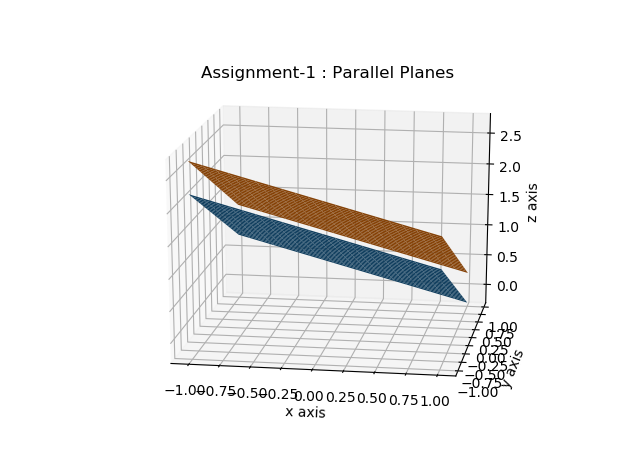
\includegraphics[width = .6\textwidth]{parallel planes.png}
\end{center}

\end{document}
